\cotefile{64}
\scanpage{40}
% archive sheet number: 39
\(\underline{\mathrm I}\unsure{c|\subset}\)

\uline{NB} \(X\mid\underline J\simeq\Delta\) est la configuration octaédrale\ldots

\diagram{\resizebox{\linewidth}{!}{\begin{tikzcd}[ampersand replacement=\&,column sep=small,row sep=small]
\begin{gathered}(X,\underline I)\ \text{\deleted{\unsure{étale|début}}}\ 
\underline I\ \text{\unsure{rev.} étale fini de degré }4\end{gathered}
\arrow[d,leftrightarrow] \& \\
\begin{gathered}
\deleted{(\underline J(\Sigma_{\underline J}),t\in\Gamma(\Sigma_J^*/S),\underline I\ \text{\deleted{rev.} torseur sous}}\\
(\underline I,\ \text{d'où }\underline J,\ t\in\Gamma(\Sigma_J^{\unsure{\alpha|*}}/S))
\end{gathered}\arrow[d,leftrightarrow]\arrow[r,leftrightarrow]\&
\begin{gathered}
\text{NB }\underline t\ \text{et }\underline I\ \text{indépendants}\\
(\underline J,\ (\text{d'où }\underline V_{\underline J}\ \text{et }\Sigma_J),\
\text{section }\inserted{t}\ \text{de }\Sigma_J^\alpha\ \text{sur }S\\
\text{torseur }I\ \text{sur }V_{\underline J})
\end{gathered}\\
\begin{gathered}
(\underline J,\ t\in\Gamma(\Sigma_{\underline J}^\alpha/S),\
X\ \text{rev. de }\Sigma_J^{\unsure{*}},\ \deleted{\unsure{g}}\ \text{étale sur }\Sigma_J^\alpha,\\
\text{jusqu'à isom sur }S,\ \text{sur chaque fibre géom. rev. \uline{abélien}}\\
\deleted{\text{de degré }4}\ \text{\inserted{\unsure{annulé|universel}, \unsure{par} \(2\)}}\ \text{\inserted{\unsure{fini|finie}, \unsure{univ.}\ldots}})\\
\text{\uline{NB} }X\ \text{et }t\ \text{sont indép. l'un de l'autre}
\end{gathered}\arrow[d,leftrightarrow] \& \\
\begin{gathered}
(\underline J,\ t\in\Gamma(\Sigma_J^\alpha/S),\ \deleted{\unsure{\underline I}}\ \underline K\ \text{torseur sous }\underline J)\\
\text{\uline{NB} }\underline K\ \text{et }t\ \text{sont indép l'un de l'autre.}
\end{gathered}\&
\end{tikzcd}}}

% margin note written sideways
\margin{\raggedright\scriptsize\(\deleted{f_i\ f_j\ f_k}\qquad x_i\ x_j\ x_k\)\\
\(V_{\underline J}(M_0)\)\\\(\unsure{V_{\underline J}(M)}\longrightarrow
\deleted{\unsure{4V_{\underline J}|\mathfrak S}}(M_0)\)\\\(\simeq\underline{\mathrm{End}}(M_0)\)\\
\(\hfill\rotatebox{90}{\(\in\)}\hspace{0.8em}\)\\
\(\hfill 1\hspace{0.8em}\)}

\hrulefill

Quand \(\underline I\) est muni d'une section, de sorte que \(\underline I\simeq\underline J\amalg S\), alors on a un iso. can \(X\simeq\Sigma_J\), d'où \(f_{\deleted{\unsure{I}}}:\Sigma_J\unsure{-|\longrightarrow}\Sigma_J\)

\scanpage{41}
% archive sheet number: 40
% letterhead
UNIVERSITE DES SCIENCES\\
ET\\
\uline{TECHNIQUES DU LANGUEDOC}\\
Service du Personnel Enseignant\\
MCS/FR.\\
N°1317.\\

Montpellier, le 9 mars 1982.\\

Le Président\\
à\\
Mesdames et Messieurs\\
les enseignants de l'U.S.T.L.\\

\uline{OBJET} : Elections au Comité Technique Paritaire Central des Personnels Enseignants de statut universitaire -\\
Scrutin par correspondance de mars 1982.\\

\uline{Réf}. : Décret n°82.139 du 5 février 1982.\\
Arrêté du 8 février 1982.\\

J'ai l'honneur de vous adresser le matériel électoral nécessaire aux opérations de vote par correspondance, comprenant :

\begin{itemize}[label={-}]
\item 1 notice explicative ;
\item 2 bulletins de vote (constitués par les listes des candidats)
\begin{itemize}[label={.}]
\item SGEN - CFDT
\item SNESUP
\end{itemize}
\item 2 professions de foi (1 pour chaque liste)
\item jeu de 3 enveloppes
\begin{itemize}[label={.}]
\item enveloppe n°1 blanche, ne comportant aucune marque ou distinction permettant d'en déterminer l'origine ;
\item enveloppe n°2 portant les mentions : nom, prénom, grade, affectation, signature ;
\item enveloppe n°3 libellée au nom de M. le Recteur, Président de la Commission de Dépouillement.
\end{itemize}
\end{itemize}

Je vous précise que les votes devront être adressés, \uline{par voie postale à M. le Recteur de l'Académie de Montpellier, la date limite de réception étant fixée au 30 mars 1982 à 17 heures,le cachet de la poste faisant foi}.

Les votes parvenus hors délais seront renvoyés aux électeurs.

Le dépouillement public se déroulera au Rectorat, Salle des Commissions, le \uline{31 mars 1982 à 14 heures}.

Le Président,\\
\handwritten{L. Thaler}\\
\uline{L. THALER}.\\

\scanpage{42}
% archive sheet number: 41
\uline{Prop} \(V\) vectoriel \unsure{dim|de} \deleted{\unsure{dég|rg}} \(2\) sur \(\mathbb F_2\), donc \(V\simeq V_J(\mathbb F_2)\), où \(J=V^*\) ens. à trois \unsure{élément|éléments}
\[
\underbrace{\operatorname{Aut}(V)}_{\Gamma}\xrightarrow{\sim}\mathfrak S_J.
\qquad\text{Posons }\operatorname{Aut}^{-}(V)\simeq\mathfrak S_J^{-}
\]
\unsure{Introduisons|Abr. d'écriture|Considérons} \(\operatorname{Aut}(V)\subset\operatorname{End}(V)=\mathcal M\deleted{\unsure{\mathrm{trice}}}\ \text{(alg. Azumaya})\).

Alors :

1) \(\deleted{\unsure{V}}\operatorname{Aut}^{-}(V)=\deleted{\unsure{W}}V'^{*}\ \deleted{\unsure{une dr}},\) où
\(\underset{\substack{\shortparallel\\\operatorname{Aut}^{-}(V)\cup\{0\}}}{V'}\subset\operatorname{End}(V)\)
est un sous-espace vectoriel de rg \(2\) canonique, can isom à \(V\), en associant à \(\deleted{\unsure{\forall|\mathrm{tt}}}\ x\in V^*\) la transposition \(\sigma_x\in\operatorname{Aut}^{-}(V)\).

2) \(\operatorname{Aut}^{+}(V)=W^{*}\), où
\(\underset{\substack{\shortparallel\\\operatorname{Aut}^{+}(V)\cup\{0\}}}{W}\subset\operatorname{End}(V)\)
est un sous-espace vectoriel de rang \(2\) canonique ;

3) \(V'\) et \(W\) sont orthogonaux l'un de l'autre pour la forme trace, qui sur \(V'\) se réduit à la forme bil. sym. unique qui est alternée et non dégénérée
\margin{\(\begin{pmatrix}0&1\\1&0\end{pmatrix}\)}
\[
\left(\operatorname{Tr}xy=
\begin{cases}
0 & \text{si }x=y,\ \text{ou }x\ \text{ou }y=0\\
1 & \text{sinon}\ \deleted{\unsure{x}}\unsure{,|;}\ \text{i.e. }x,y\in V'^{*},\ \unsure{a|x}\ne y
\end{cases}\right),
\]
et sur \(W\) est non alternée \((\operatorname{Tr}\rho^2=\operatorname{Tr}\rho^{-2}=1,\ \operatorname{Tr}1^2=0)\)
\margin{\(\begin{pmatrix}1&0\\0&1\end{pmatrix}\)}
et bien sur non dégénérée.

\figure{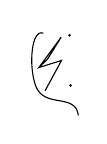
\begin{tikzpicture}[x=.32cm,y=.32cm]
\draw (0.55,2.9) .. controls (0.08,3.1) and (-.05,1.6) .. (.25,.8) .. controls (.6,-.1) and (1.82,.55) .. (1.94,-.36);
\draw (.38,1.55)--(1.26,2.75)--(.72,1.88)--(.37,1.54)--(1.27,1.82)--(.62,.62);
\fill (1.59,2.82) circle (.057) (1.63,.83) circle (.055);
\end{tikzpicture}}

4) \(V'\) \deleted{\unsure{qui est}} en tant que \(\mathbb F_2(\Gamma)\)-module est isom. à \(V\) et irréductible, tandis que \(W\) est une extension non scindée
\diagram{\begin{tikzcd}[ampersand replacement=\&,column sep=small]
0\arrow[r]\&\mathbb F_2\arrow[r,"\lambda\longmapsto\lambda.1"']\&W\arrow[r,"\operatorname{Tr}"']\&\mathbb F_2\arrow[r]\&0
\end{tikzcd}}
\margin{\uline{NB} \(\mathbb F_2.1\) est son propre orthogonal}
\hfill TSVP

\scanpage{43}
% archive sheet number: 42
5) On a
\[
\unsure{\mathfrak{sl}(V)|\mathrm{sl}(V)}
\overset{\mathrm{def}}{=}
\operatorname{Ker}\bigl(M\xrightarrow{\operatorname{Tr}}\mathbb F_2\bigr)
=V'+\mathbb F_2.1_V
\]

\scanpage{44}
% archive sheet number: 43
\margin{(25 \unsure{v|p})}
II \qquad Structure octaédrale dans \(\mathbb P^1\)

\scanpage{45}
% archive sheet number: 44
\mspage{1}
\begingroup\csname tagsleft@true\endcsname
1. Opération de groupes \(\simeq\mathbb D_2\) sur la droite projective, et configuration octaédrale.

Soit \(V\) un groupe qui est un espace vectoriel de rang \(2\) sur \(\mathbb F_2\), \deleted{\unsure{?}} et considérons un\deleted{e droite pro} fibré en droites projectives \(X\) sur un schéma de base \(S\). On s'intéresse aux opérations, fidèles sur chaque fibre, de \(V\) sur \(X\), i.e. aux monomorphismes
\[
V_S\lhook\joinrel\longrightarrow\underline{\operatorname{Aut}}_S(X)=G \tag*{(1)}
\]
Choisissons une base \(e_1,e_2\) de \(V\) sur \(\mathbb F_{\unsure{1|2}}\), alors la donnée d'un hom
\[
V_S\longrightarrow\underline{\operatorname{Aut}}_S(X)\qquad\text{i.e.}\quad V\longrightarrow\operatorname{Aut}_S(X)
\]
qui soit mono sur \(\mathbb F_2 e_1\) et sur \(\mathbb F_2 e_2\), équivaut à celle de \inserted{\unsure{autom|autom.} d'ordre deux de \(X\), ou encore de} deux ``axes'' (ou diviseurs étales de degré \(2\)) \(\Delta_1,\Delta_2\) sur \(X\), la condition de commutation étant que \(\Delta_2\) est stable par \(\sigma_1\), ou \deleted{\unsure{en}} encore \(\Delta_1\) stable par \(\sigma_2\).
% slanted
\margin{on est en car. \(\ne2\)\\
\(\Delta_1=X^{\sigma_1}\)\\
\(\unsure{\Delta_2}=X^{\sigma_2}\)}
\deleted{Pour \(\sigma_1\) donné i.e. \(\Delta_1\) donné, \unsure{i.e. de \(\Delta_2\)} la donnée de \(\sigma_2\) \unsure{revient}} \inserted{La condition que (1) soit un mono signifie} \deleted{\unsure{que}} \unsure{aussi} que l'on ; \deleted{donc \unsure{à la donnée|que la donnée} d'une section de \(X/\{1,\sigma_1\}\unsure{\to|-}\)}
\[
\Delta_1\cap\Delta_2=\varnothing\qquad\text{i.e.}\quad\Delta_2\subset X-\Delta_1 \tag*{(2)}
\]
et pour \(\sigma_1\) \inserted{i.e. \(\Delta_1\)} donné, la donnée de \(\deleted{\unsure{e_2}}\ \sigma_2\) i.e. de \(\Delta_2\) équivaut à celle d'une section de \deleted{\unsure{\(X-\Delta_1\) sur|\(\Delta_1\) sur}} \((X-\Delta_1)/\{1,\sigma_1\}\) sur \(S\) (\(\Delta_2\) étant alors l'image inverse de cette section dans \(X-\Delta_1\)). Considérons le troisième larron \(e\)
\[
e_3=e_1+e_2 \tag*{(3)}
\]
il lui correspond un axe \(\Delta_3\), et \(\Delta_1,\Delta_2,\Delta_3\) sont mutuellement disjoints.
\endgroup

\scanpage{46}
% archive sheet number: 45
\begingroup\csname tagsleft@true\endcsname
\(\cdot\) La donnée de \(\Delta_1\) est unique à conjugaison locale près -- si on prend une trivialisation de \deleted{\unsure{droite de \(X\) sur}} \(\Delta_1\), \deleted{on peut prendre} la situation \((X,\Delta_1)\) i.e. \deleted{\unsure{se}} est isom. localement à \((\mathbb P^1_S,\{0,\infty\})\), \(\sigma_1\) étant donné par \(z\mapsto-z\), donc \(X\setminus\Delta_1\) étant \(\deleted{\unsure{G_m}}\ \mathbb P^1_S\setminus\{0,\infty\}=\mathbb G_{mS}\), et le quotient \((X\setminus\Delta_1)/\{1,\sigma_1\}\), s'identifiant à \(\mathbb G_{mS}\), l'hom de passage au quotient étant
\diagram{\begin{tikzcd}[ampersand replacement=\&,row sep=.15em]
X\setminus\Delta_1\arrow[r]\&(X\setminus\Delta_1)/\{1,\sigma_1\}\\
\rotatebox{90}{\(\simeq\)}\&\rotatebox{90}{\(\simeq\)}\\
\mathbb G_{mS}\arrow[r,"\lambda\mapsto\lambda^2"]\&\mathbb G_{mS}
\end{tikzcd}}

La donnée d'une section de \((X\setminus\Delta_1)/\{1,\sigma_1\}\) équivaut alors à celle d'une section \(\lambda\) de \(\mathbb G_{mS}\) -- et loc pour la top. étale, on peut poser \(\lambda=\unsure{\zeta|\xi}^2\), \deleted{et quitte à remplacer} \inserted{i.e. \deleted{\unsure{que}} la section} \deleted{\unsure{la}} \(\lambda\) provient d'une section \(\zeta\) de \(X\setminus\Delta_1\) sur \(S\). On peut (quitte à remplacer l'iso. \(X\simeq\mathbb P^1_S\) par un autre, savoir son multiple par \(1/\zeta\)) supposer que \unsure{c'est|\(\zeta\) est|\(\xi\) est} la section \(1\), de sorte que la situation \unsure{standart|standard} est
\[
\left\{\begin{aligned}
\Delta_1&=\{0,\infty\},&\Delta_2&=\{1,-1\}\\
\sigma_1(z)&=-z&\sigma_2(z)&=\frac1z
\end{aligned}\right. \tag*{(4)}
\]
(NB \(\sigma_2\) est l'unique homographie qui échange \(0\) et \(\infty\), et fixe \(1\) et \(-1\)). On trouve alors
\endgroup

\scanpage{47}
% archive sheet number: 46
\mspage{2}
\begingroup\csname tagsleft@true\endcsname
\[
\begin{aligned}
\sigma_3(z)&=-\frac1z & \Delta_3&=\mathbb V(z^2+1)\ \bigl(=\{i,-i\}\\
&&&\text{si }\exists\ \text{racine primitive}\\
&&&\text{de }\unsure{\varepsilon|4}{-1}\ \text{sur }S\bigr)
\end{aligned} \tag*{(5)}
\]
On trouve donc

\uline{Proposition} Loc pour la top. étale, une représentation monomorphique de \(\mathbb D_4=\mathbb F_2\times\mathbb F_2\) dans \(\operatorname{Aut}(\mathbb P^1_S)\) (sur une base \(S\) à car. résid. \(\ne2\)) est donnée par (4) (\deleted{où} \(\sigma_1,\sigma_2\) sont les autos correspondant aux éléments de la base canonique \((e_1,e_2)\) de \(\mathbb D_4\) sur \(\mathbb F_2\)) -- qui donne bien une représentation monomorphique.

Posons
\[
\begin{aligned}
\Delta&=\Delta_1\amalg\Delta_2\amalg\Delta_3\qquad\bigl(=\{0,\infty,1,-1,i,-i\}\\
&\hspace{14em}\text{dans le cas normalisé}\bigr)
\end{aligned} \tag*{(6)}
\]
on appelle \(\Delta\) la \uline{configuration octaédrale} associée à l'opération de \(V\) sur \deleted{\unsure{\(e\)}} \(X\) -- par descente plate, elle est définie comme diviseur étale de degré \(6\) de \(X/S\)) dès qu'on a une opération monomorphique \inserted{(sur chaque fibre)} d'un groupe \(V\) \inserted{\(\simeq\mathbb D_4\)} sur \(X\), ou plus généralement d'un schéma en groupes \(\underline V\) sur \(S\) loc. isom. au schéma en groupes constant. \deleted{\unsure{Alors}} De façon générale, on appelle \uline{configuration octaédrale} dans \(X/S\) un diviseur étale de degré \(6\) de \(X/S\), qui soit
\endgroup

\scanpage{48}
% archive sheet number: 47
\begingroup\csname tagsleft@true\endcsname
loc. isomorphe à \(\{0,\infty,1,-1,i,-i\}\) de \(\mathbb P^1_S\), ou ce qui revient au \(=\), qui soit loc. isom. à la configuration octaédrale associée à une op. \inserted{\unsure{monom.}} d'un \(\underline V\) sur \(X\). Nous allons voir maintenant que cette donnée est essentiellement unique.

Pour ceci, pour un diviseur octaédral \(\deleted{\unsure{\Delta}}\)
\[
\Delta\subset X
\]
considérons le schéma en groupes
\[
\deleted{\unsure{G}}\Gamma=\underline{\operatorname{Aut}}_{\Delta}(X,\Delta), \tag*{(7)}
\]
Il est immédiat (du fait que \(\Delta\) est de degré \(\geq3\)) que \(\Gamma\) est \uline{net} sur \(S\), \inserted{car \(\subset\underline{\mathfrak S}_{\Delta}=\underline{\operatorname{Aut}}_S(\Delta)\)} Je dis que \(\Gamma\) est étale sur \(S\), et loc. isom au schéma en groupes \((\mathfrak S_4)_S\). Plus précisément, je vais définir sur \(\Delta\) \inserted{(comme schéma des sommets)} une structure d'o\deleted{\unsure{ct}} schéma en octaèdres combinatoires; de telle façon que l'on ait
\[
\begin{aligned}
\Gamma&=\underline{\operatorname{Aut}}^{+}_{\mathrm{oct.}}(\Delta)
\qquad\bigl(\text{en tant que}\\
&&\text{sous-schémas de}\\
&&\underline{\operatorname{Aut}}_S(\Delta)\bigr)
\end{aligned} \tag*{(8)}
\]
Pour ceci, on \deleted{\unsure{va décrire une}} \inserted{note qu'une} structure octaédrale sur un ens. à six éléments \(\Delta\) est bien déterminée quand on connaît le groupe de ses automorphismes \inserted{directs} (en tant que \unsure{sous-groupes|sous-groupe} de \(\mathfrak S_{\Delta}\)), car
\endgroup

\scanpage{49}
% archive sheet number: 48
\mspage{3}
les ``diagonales'' \(\Delta_1,\Delta_2,\Delta_3\) de \(\Delta\) sont déterminées \deleted{par la condition que leur stabilisateur soit} \inserted{(en tant que parties à deux éléments de \(\Delta\))} comme les classes pour la relation d'équivalence \(R\) définie par l'application \(s\mapsto\Gamma_s\) (\(s\) et \(s'\) sont dans une \(=\) classe ssi ils ont le \(=\) groupe d'isotropie, qui est \inserted{cyclique} d'ordre \(4\)), et la structure polyédrale est déterminée en termes de cette décomposition \inserted{de \(\Delta\)}, les arêtes étant les \inserted{12} parties à deux éléments distinctes des \(\Delta_i\), et les \inserted{8} faces étant les parties à trois éléments \uline{sections} de \(\Delta\longrightarrow\Delta/R\).

Donc la structure octaédrale sur \(\Delta\) revient à la structure \deleted{\unsure{de}} définie par \(R\), relation d'équivalence de degré \(2\), ou \unsure{encore|aussi} par celle du groupe \(\Gamma\) (\(\simeq\mathfrak S_4\)) opérant sur \(\Delta\).

Cette parenthèse combinatoire montre que la structure octaédrale \unsure{annoncée|canonique} sur \(\Delta\subset X\) est nécessairement unique (puisqu'on connaît son schéma en groupes d'autom.), ce qui montre que la question d'existence est locale (\unsure{ét|ét.}), donc OPS \(X=\mathbb P^1_S,\ \Delta=\{0,\infty,1,-1,i,-i\}\). Le \deleted{stabilisateur de \(0,\infty\)} \inserted{sous-groupe de} \(\deleted{\unsure{G|\Gamma}}\Gamma\) qui fixe \(0\) et \(\infty\) est isomorphe visiblement à \(\mu_4\deleted{\unsure{\simeq}}\simeq(\mathbb Z/4\mathbb Z)_S\) (générateur \(i\)), \deleted{et par} et de \(=\) (par raison d'homogénéité) pour \((1,-1)\), \((i,-i)\). Par contre, le

\scanpage{50}
% archive sheet number: 49
groupe des autom. de \((X,\Delta)\) qui fixe \(\infty\) et \(-1\) donc \inserted{des \unsure{autos|autom.}} de la forme \(z\mapsto az+b\) avec \(-a+b=-1\)
\[
\text{i.e.}\qquad z\longmapsto\deleted{a(z-1)+1=az+(1-a)}az+(a-1)
\]
est plus petit, en fait si l'autom envisagé n'est pas l'identité, il doit induire une permutation sans pts fixes de \((0,1,i,-i)\), qui est donc d'ordre \(2\) ou quatre, donc on a \(a^4=1\) \deleted{ou \(a^4=1\)} \deleted{i.e. \(a\in\{0,1,i,\unsure{-}\)} mais faisant \(z=0\) on doit avoir
\[
a-1\in\{1,i,-i\}\qquad\text{i.e.}\quad a\in(2,1+i,1-i)
\]
% slanted
\margin{donc \(a^4=\pm4\) qui ne peut être \(=1\) qu'en car \(3\) et \(5\)}
faisant \(z=1\) on trouve
\[
2a-1\in\{0,i,-i\}\qquad\text{i.e.}\quad
a\in\{1/2,\tfrac12(i+1),\tfrac12(1-i)\}
\]
% slanted
\margin{donc \(a^4=1/4\) ou \(a^4=-1\) qui n'est pas égal à \(1\) (car on est en car \(\ne2\))}
\(\bigl[\)faisant \(z=i\), on trouve
\[
a\underbrace{(i+1)}_{1:\left(\frac{1-i}{2}\right)}-1\in\{0,1,-i\}\qquad\text{i.e.}\quad
a\in\left\{\frac{1\deleted{\unsure{+}}\unsure{-}i}{\deleted{\unsure{4}}2},\deleted{\unsure{\frac{2}{1+i}}}1-i,-i\right\}
\]
et de \(=\), faisant \(z=-i\), on trouve
\[
a\in\left\{\frac{1+i}{2},1+i,i\right\}\biggr]
\]
Donc l'\deleted{\unsure{a}}intersection des stabilisateurs de \(\infty,-1\) est \(\{1\}\), et par raison d'homogénéité il en est de \(=\) pour \deleted{\unsure{tout|toute}} partie à deux éléments de \(\Delta\), distincte de \(\Delta_1,\Delta_2,\Delta_3\). Donc on voit que la structure octaédrale \(\Delta=\Delta_1\amalg\Delta_2\amalg\Delta_3\) est invariante par \(\Gamma\), et uniquement déterminée par le diviseur \(\Delta\). Donc \(\Gamma\hookrightarrow\underline{\operatorname{Aut}}_{\mathrm{oct}}(\Delta)\),
% slanted
\margin{et on a \(=\)\\ \(\Gamma\subset\operatorname{Aut}^{+}_{\mathrm{oct}}(\Delta)\)}
Pour montrer qu'on a \unsure{isomorphisme|isomorphie}, il suffit de noter que le groupe des autom \inserted{directs} de la structure octaédrale est engendrée par les trois sous-groupes cycliques d'ordre \(4\) \deleted{\unsure{\(t_1=\)}} qu'il contient, correspondants à \(\Delta_1,\Delta_2,\Delta_3\) -- or ceux-ci sont contenus dans \(\Gamma\).

\scanpage{51}
\mspage{4}
Soit \(\Delta\) un diviseur étale de degré \(6\) dans \(X/S\), muni d'une structure octaédrale i.e. d'une \deleted{\unsure{projection} \unsure{finie}} \deleted{de degré \(2\)} \inserted{opération involutive}
\[
 \deleted{\Delta\longrightarrow\Delta'}\quad \underline{a}_{\Delta}:\Delta\longrightarrow\Delta
\]
\deleted{\unsure{où|i.e.} \(\Delta'\) est fini étale de degré \(3\) sur \(S\).} correspondant à une opération libre de \(\{1,\underline{a}_{\Delta}\}\) sur \(\Delta/S\). On dit que cette structure octaédrale est \deleted{\uline{\unsure{homogène}}, \unsure{si}} \inserted{\uline{régulière} dans} \(X\), si le groupe \(\Gamma=\underline{\operatorname{Aut}}_{\rm oct}^{+}(\Delta)\) opère sur \(X\), de façon compatible avec les op. sur \(\Delta\) (cette op de \(\Gamma\) sur \(X\) est alors unique).
% slanted
\margin{Il faut un petit argument pour montrer que tout \unsure{autom|autom.} de la structure oct. \unsure{de} \(\Delta\) induit par un autom de \((X,\Delta)\) est direct : OPS que l'autom fixe les points de \(\{0,\infty\}=\Delta_1\), et on trouve \unsure{alors|dans} les autom de ``\unsure{rotations|rotation}'' par \(\mu_4\), qui sont bien directs\ldots}

\deleted{\unsure{P|Pour}} Pour \(\Delta\) \inserted{diviseur} fixé, on voit qu'il y a au plus une structure octaédrale sur \(\Delta\) qui soit régulière, et il y en a une ssi \(\Delta\) est une ``configuration octaédrale''. Si \(\Delta\) est une telle configuration, on vient de voir \inserted{déjà} qu'elle est munie d'une \deleted{unique} structure octaédrale, régulière (et \uline{tout} autom. de \(X\) qui \deleted{fixe} \inserted{\unsure{invarie|conserve|respecte}} \(\Delta\) \deleted{fixe} \inserted{\unsure{invarie|conserve|respecte}} cette structure octaédrale).
% slanted
\margin{Si on a une configuration octaédrale régulière \(\deleted{\Delta}\) dans un fibré en droites projectives \(X\), alors le revêtement des orientations de \(\Delta\) est can. isom. au revêtement \(\mu_4^{*}\) \deleted{\unsure{de|\(=\)}} \(\operatorname{Spec}\mathcal O_S[i]\unsure{u}/(i^2+1)\) de \(S\)\ldots}
Inversement, si \(\Delta\) est muni d'une str. oct. rég, alors le sous-groupe \(\underline V\) de \(\underline\Gamma=\underline{\operatorname{Aut}}\deleted{\unsure{\rm oct}}_{\rm oct}(\Delta)\) inv. abélien non trivial est un groupe \deleted{loc.} isom. à \(\mathbb D_{2S}\), opérant fidèlement sur \(X\), et on voit aussitôt que \unsure{la|le}
% archive sheet number: 50

\scanpage{52}
configuration \deleted{\unsure{icosaèdre|icosaédrale}} \inserted{octaédrale} associée est bien celle de départ\ldots

\uline{Théorème} \quad Soit \(X\) un fibré en droites projectives sur un schéma \(S\), de car. \deleted{\unsure{rési}} résiduelles \(\ne 2\). Considérons le \deleted{\unsure{grp}} schéma en groupes \(G=\underline{\operatorname{Aut}}_S(X)\) (\uline{NB} la donnée de \(X/S\) équivaut à celle de la ``forme'' \(G\) de \(\mathrm{GP}(1)_S\) sur \(S\)), et les ensembles suivants :

a) L'ens \(\mathcal A(X)\) des sous-schémas en groupes \(V\) de \(G\), loc isom. à \((\mathbb D_4)_S\)

b) L'ens \deleted{\unsure{de|a}} \(\mathcal B(X)\) des sous-schémas en groupes \(\deleted{\unsure{\mathfrak S|G}}\Gamma\) de \(G\), loc. isom. à \((\mathfrak S_4)_S\).

c) L'ens des configurations icosaédrales régulières dans \(X\), i.e. des diviseurs étales \(\Delta\) dans \(X/S\), de degré \(6\), munis de un antipodisme \(\underline a_\Delta:\Delta \mathbin{\text{---}} \Delta\) qui \deleted{\unsure{définit un autom.}} \inserted{\unsure{soit|sont} sans pts} fixe sur chaque fibre géom., et tel que \(\underline{\operatorname{Aut}}_{\unsure{S,\rm oct|\rm oct}}^+(\deleted{\unsure{X}}\Delta)\) opère sur \(X\) de façon compatible avec son opération sur \(\Delta\).

On a alors un système transitif de bijections canoniques entre ces trois ensembles, \unsure{obtenues|obtenus|obtenu} ainsi !
% archive sheet number: 51
